% !TEX root = ../../main.tex
\chapter{Thiết kế Logic (Logical Design)}
\label{chap:chuong2_logic}

Giai đoạn thiết kế logic thực hiện chuyển đổi mô hình Thực thể -- Kết hợp trừu tượng thành Lược đồ quan hệ (Relational Schema) tương thích với mô hình dữ liệu quan hệ, tiến hành chuẩn hóa dữ liệu để triệt tiêu dị thường và trực quan hóa toàn bộ mạng lưới cấu trúc dữ liệu thông qua Sơ đồ ERD ở mức logic.

% !TEX root = ../../main.tex
\section{Quy tắc chuyển đổi từ mô hình ER sang mô hình quan hệ (Relational Model)}
\label{sec:2_1_quy_tac_chuyen_doi}

Chuyển đổi từ mô hình Thực thể -- Liên kết mở rộng (ERD/EERD) sang Mô hình Quan hệ (Relational Model) là bước then chốt trong giai đoạn Thiết kế Logic (Logical Design). Quá trình này đảm bảo toàn bộ thông tin, ràng buộc dữ liệu và mối quan hệ giữa các đối tượng trong hệ thống \textbf{FamilyConnect} được biểu diễn chính xác, toàn vẹn dưới dạng các lược đồ quan hệ (Relation Schemas).

Hệ thống chuyển đổi từ \textbf{17 thực thể nghiệp vụ quan niệm} sang tập hợp \textbf{22 lược đồ quan hệ logic} thông qua 4 quy tắc kỹ thuật chuẩn hóa:
\begin{enumerate}
    \item \textbf{10 Thực thể mạnh} $\longrightarrow$ \textbf{10 Bảng chính} (Primary Tables).
    \item \textbf{5 Thực thể phụ thuộc tồn tại} $\longrightarrow$ \textbf{5 Bảng phụ} (Dependent Tables với FK \texttt{NOT NULL} và \texttt{ON DELETE CASCADE}).
    \item \textbf{5 Mối kết hợp $M{:}N$} $\longrightarrow$ \textbf{5 Bảng trung gian} (Junction Tables).
    \item \textbf{1 Phân cấp chuyên biệt hóa (EER)} $\longrightarrow$ \textbf{2 Bảng kế thừa thực thể con}\newline (\texttt{thanh\_vien\_noi\_toc}, \texttt{thanh\_vien\_dau\_re}).
\end{enumerate}

% Macro tự động co giãn nội dung nếu tràn ô trong bảng
\newlength{\tblcellwd}
\newcommand{\tblcellfit}[1]{%
    \settowidth{\tblcellwd}{\small#1}%
    \ifdim\tblcellwd>\linewidth
        \resizebox{\linewidth}{!}{#1}%
    \else
        \small#1%
    \fi
}

\subsection{Chuyển đổi thực thể mạnh thành Bảng chính}
\label{subsec:2_1_1_chuyen_doi_thuc_the}

Mỗi thực thể mạnh trong mô hình ERD tương ứng với một bảng chính trong mô hình quan hệ. Các thuộc tính đơn trở thành các cột của bảng, và thuộc tính định danh được chọn làm Khóa chính (Primary Key -- PK). Quy ước đặt tên bảng và cột theo chuẩn \texttt{snake\_case}.

\setlength{\arrayrulewidth}{0.65pt}
\renewcommand{\arraystretch}{1.55}

\begin{longtable}{|c|p{2.8cm}|>{\raggedright\arraybackslash}p{3.5cm}|p{5.7cm}|}

    \caption{Chuyển đổi 10 Thực thể mạnh thành Bảng chính}
    \label{tab:2_1_1_thuc_the_manh}\\

    \hline
    \rowcolor{tableheader}
    \centering\textcolor{white}{\textbf{STT}} &
    \centering\textcolor{white}{\textbf{Thực thể (ERD)}} &
    \centering\textcolor{white}{\textbf{Bảng CSDL (\texttt{snake\_case})}} &
    \textcolor{white}{\textbf{Ghi chú thiết kế}}\tabularnewline
    \hline
    \endfirsthead
    \multicolumn{4}{l}{\small\textit{(tiếp Bảng~\ref{tab:2_1_1_thuc_the_manh})}}\\[2pt]
    \hline
    \rowcolor{tableheader}
    \centering\textcolor{white}{\textbf{STT}} &
    \centering\textcolor{white}{\textbf{Thực thể (ERD)}} &
    \centering\textcolor{white}{\textbf{Bảng CSDL (\texttt{snake\_case})}} &
    \textcolor{white}{\textbf{Ghi chú thiết kế}}\tabularnewline
    \hline
    \endhead
    \hline
    \endlastfoot

    % ---- Nhóm 1: User & Security ----
    \multicolumn{4}{|l|}{\small\textit{\textbf{Phân hệ 1: Người dùng \& Bảo mật (User \& Security)}}}\\
    \hline

    1 &
    \small NguoiDung &
    \tblcellfit{\texttt{nguoi\_dung}} &
    \small Khóa chính (PK): \texttt{ma\_nguoi\_dung} (UUID). Quản lý tài khoản đăng nhập hệ thống.\\
    \hline

    \rowcolor{tablerowalt}
    2 &
    \small VaiTro &
    \tblcellfit{\texttt{vai\_tro}} &
    \small Khóa chính (PK): \texttt{ma\_vai\_tro} (UUID). Định nghĩa các vai trò RBAC.\\
    \hline

    3 &
    \small Quyen &
    \tblcellfit{\texttt{quyen}} &
    \small Khóa chính (PK): \texttt{ma\_quyen} (UUID). Danh mục các quyền thao tác nghiệp vụ.\\
    \hline

    % ---- Nhóm 2: Family & Genealogy ----
    \multicolumn{4}{|l|}{\small\textit{\textbf{Phân hệ 2: Gia tộc \& Gia phả (Family \& Genealogy)}}}\\
    \hline

    4 &
    \small DongHo &
    \tblcellfit{\texttt{dong\_ho}} &
    \small Khóa chính (PK): \texttt{ma\_dong\_ho} (UUID). Đại dòng họ, đỉnh cao nhất của phả hệ.\\
    \hline

    \rowcolor{tablerowalt}
    5 &
    \small ChiToc &
    \tblcellfit{\texttt{chi\_toc}} &
    \small Khóa chính (PK): \texttt{ma\_chi\_toc} (UUID). FK: \texttt{ma\_dong\_ho} tham chiếu \texttt{dong\_ho}.\\
    \hline

    6 &
    \small ThanhVien &
    \tblcellfit{\texttt{thanh\_vien}} &
    \small Khóa chính (PK): \texttt{ma\_thanh\_vien} (UUID). FK: \texttt{ma\_chi\_toc}, \texttt{ma\_nguoi\_dung}, \texttt{ma\_cha}, \texttt{ma\_me}.\\
    \hline

    % ---- Nhóm 3: Community & Events ----
    \multicolumn{4}{|l|}{\small\textit{\textbf{Phân hệ 3: Tương tác, Sự kiện \& Truyền thông (Community \& Events)}}}\\
    \hline

    \rowcolor{tablerowalt}
    7 &
    \small BaiViet &
    \tblcellfit{\texttt{bai\_viet}} &
    \small Khóa chính (PK): \texttt{ma\_bai\_viet} (UUID). FK: \texttt{ma\_nguoi\_tao} tham chiếu \texttt{nguoi\_dung}.\\
    \hline

    8 &
    \small AlbumAnh &
    \tblcellfit{\texttt{album\_anh}} &
    \small Khóa chính (PK): \texttt{ma\_album} (UUID). FK: \texttt{ma\_thanh\_vien} tham chiếu \texttt{thanh\_vien}.\\
    \hline

    \rowcolor{tablerowalt}
    9 &
    \small SuKien &
    \tblcellfit{\texttt{su\_kien}} &
    \small Khóa chính (PK): \texttt{ma\_su\_kien} (UUID). FK: \texttt{ma\_nguoi\_tao} tham chiếu \texttt{nguoi\_dung}.\\
    \hline
    % ---- Nhóm 4: Heritage ----
    \multicolumn{4}{|l|}{\small\textit{\textbf{Phân hệ 4: Di sản số (Family Heritage)}}}\\
    \hline

    10 &
    \small DiSanLichSu &
    \tblcellfit{\texttt{di\_san\_lich\_su}} &
    \small Khóa chính (PK): \texttt{ma\_di\_san} (UUID). FK: \texttt{ma\_thanh\_vien} tham chiếu \texttt{thanh\_vien}.\\
    \hline

\end{longtable}

\renewcommand{\arraystretch}{1.0}
\setlength{\arrayrulewidth}{0.4pt}

\subsection{Chuyển đổi thực thể phụ thuộc tồn tại thành Bảng phụ}
\label{subsec:2_1_2_chuyen_doi_thuc_the_yeu}

Thực thể phụ thuộc tồn tại (\textit{Existence-dependent Entities}) phụ thuộc chặt chẽ vào thực thể chủ. Nhằm đảm bảo hiệu năng và chuẩn hóa CSDL quan hệ hiện đại, các bảng phụ tương ứng được cấu hình:
\begin{itemize}
    \item \textbf{Khóa chính đại diện (Surrogate PK):} Dùng kiểu UUID tự sinh để hỗ trợ liên kết nhanh và đánh chỉ mục độc lập.
    \item \textbf{Khóa ngoại bắt buộc (FK \texttt{NOT NULL}):} Trỏ về bảng chính chủ. Đối với quan hệ $1:1$ (như Hồ sơ nghề nghiệp, Danh nhân), cột FK mang ràng buộc \texttt{UNIQUE}.
    \item \textbf{Chính sách xóa thác lũ (\texttt{ON DELETE CASCADE}):} Khi bản ghi chủ bị xóa, các bản ghi phụ thuộc tự động bị loại bỏ để đảm bảo tính toàn vẹn tham chiếu.
\end{itemize}

\setlength{\arrayrulewidth}{0.65pt}
\renewcommand{\arraystretch}{1.55}

\begin{longtable}{|c|p{2.8cm}|>{\raggedright\arraybackslash}p{3.5cm}|p{5.7cm}|}

    \caption{Chuyển đổi 5 Thực thể phụ thuộc tồn tại thành Bảng phụ}
    \label{tab:2_1_2_thuc_the_yeu}\\

    \hline
    \rowcolor{tableheader}
    \centering\textcolor{white}{\textbf{STT}} &
    \centering\textcolor{white}{\textbf{Thực thể phụ thuộc}} &
    \centering\textcolor{white}{\textbf{Bảng phụ (\texttt{snake\_case})}} &
    \textcolor{white}{\textbf{Ghi chú thiết kế}}\tabularnewline
    \hline
    \endfirsthead
    \multicolumn{4}{l}{\small\textit{(tiếp Bảng~\ref{tab:2_1_2_thuc_the_yeu})}}\\[2pt]
    \hline
    \rowcolor{tableheader}
    \centering\textcolor{white}{\textbf{STT}} &
    \centering\textcolor{white}{\textbf{Thực thể phụ thuộc}} &
    \centering\textcolor{white}{\textbf{Bảng phụ (\texttt{snake\_case})}} &
    \textcolor{white}{\textbf{Ghi chú thiết kế}}\tabularnewline
    \hline
    \endhead
    \hline
    \endlastfoot

    1 &
    \small NhatKyHeThong &
    \tblcellfit{\texttt{nhat\_ky\_he\_thong}} &
    \small PK: \texttt{ma\_nhat\_ky}. FK: \texttt{ma\_nguoi\_dung} $\to$ \texttt{nguoi\_dung} (\texttt{CASCADE}).\\
    \hline

    \rowcolor{tablerowalt}
    2 &
    \tblcellfit{HoSoNgheNghiep} &
    \tblcellfit{\texttt{ho\_so\_nghe\_nghiep}} &
    \small PK: \texttt{ma\_ho\_so}. FK: \texttt{ma\_thanh\_vien} $\to$ \texttt{thanh\_vien} (\texttt{CASCADE}, \texttt{UNIQUE} ép quan hệ 1:1).\\
    \hline

    3 &
    \small BinhLuan &
    \tblcellfit{\texttt{binh\_luan}} &
    \small PK: \texttt{ma\_binh\_luan}. FK: \texttt{ma\_bai\_viet} $\to$ \texttt{bai\_viet} (\texttt{CASCADE}); FK: \texttt{ma\_thanh\_vien} $\to$ \texttt{thanh\_vien} (\texttt{SET NULL}).\\
    \hline

    \rowcolor{tablerowalt}
    4 &
    \small NhanVatTieuBieu &
    \tblcellfit{\texttt{nhan\_vat\_tieu\_bieu}} &
    \small PK: \texttt{ma\_nhan\_vat}. FK: \texttt{ma\_thanh\_vien} $\to$ \texttt{thanh\_vien} (\texttt{CASCADE}, \texttt{UNIQUE} ép quan hệ 1:1).\\
    \hline

    5 &
    \small ThongBao &
    \tblcellfit{\texttt{thong\_bao}} &
    \small PK: \texttt{ma\_thong\_bao}. FK: \texttt{ma\_nguoi\_dung} $\to$ \texttt{nguoi\_dung} (\texttt{CASCADE}). Lưu thông báo hệ thống.\\
    \hline

\end{longtable}

\renewcommand{\arraystretch}{1.0}
\setlength{\arrayrulewidth}{0.4pt}

\subsection{Chuyển đổi các mối quan hệ 1--1, 1--N, N--N và mối quan hệ đệ quy}
\label{subsec:2_1_3_chuyen_doi_moi_quan_he}

\subsubsection{Ánh xạ Quan hệ 1:1 và 1:N (Chèn Khóa ngoại FK)}

Với quan hệ \textbf{1:1} và \textbf{1:N}, Khóa chính của bảng phía \textbf{1/Chính} được chèn vào bảng phía \textbf{N/Phụ} dưới dạng Khóa ngoại (FK). Riêng quan hệ 1:1 bắt buộc có ràng buộc \texttt{UNIQUE} trên cột FK để bảo đảm tính đơn nhất.

\setlength{\arrayrulewidth}{0.65pt}
\renewcommand{\arraystretch}{1.55}

\begin{longtable}{|c|>{\raggedright\arraybackslash}p{3.2cm}|>{\raggedright\arraybackslash}p{3.0cm}|p{2.8cm}|p{2.2cm}|}

    \caption{Ánh xạ Quan hệ 1:1 và 1:N -- Chèn Khóa ngoại FK}
    \label{tab:2_1_3_fk_mapping}\\

    \hline
    \rowcolor{tableheader}
    \centering\textcolor{white}{\textbf{STT}} &
    \centering\textcolor{white}{\textbf{Bảng chứa FK (Phía N/Phụ)}} &
    \centering\textcolor{white}{\textbf{Cột FK được chèn}} &
    \centering\textcolor{white}{\textbf{Bảng đích (Phía 1/Chính)}} &
    \textcolor{white}{\textbf{Loại quan hệ}}\tabularnewline
    \hline
    \endfirsthead
    \multicolumn{5}{l}{\small\textit{(tiếp Bảng~\ref{tab:2_1_3_fk_mapping})}}\\[2pt]
    \hline
    \rowcolor{tableheader}
    \centering\textcolor{white}{\textbf{STT}} &
    \centering\textcolor{white}{\textbf{Bảng chứa FK (Phía N/Phụ)}} &
    \centering\textcolor{white}{\textbf{Cột FK được chèn}} &
    \centering\textcolor{white}{\textbf{Bảng đích (Phía 1/Chính)}} &
    \textcolor{white}{\textbf{Loại quan hệ}}\tabularnewline
    \hline
    \endhead
    \hline
    \endlastfoot

    1 &
    \tblcellfit{\texttt{thanh\_vien}} &
    \tblcellfit{\texttt{ma\_nguoi\_dung}} &
    \tblcellfit{\texttt{nguoi\_dung}} &
    \small 1:1 (\texttt{UNIQUE})\\
    \hline

    \rowcolor{tablerowalt}
    2 &
    \tblcellfit{\texttt{chi\_toc}} &
    \tblcellfit{\texttt{ma\_dong\_ho}} &
    \tblcellfit{\texttt{dong\_ho}} &
    \small 1:N\\
    \hline

    3 &
    \tblcellfit{\texttt{thanh\_vien}} &
    \tblcellfit{\texttt{ma\_chi\_toc}} &
    \tblcellfit{\texttt{chi\_toc}} &
    \small 1:N\\
    \hline

    \rowcolor{tablerowalt}
    4 &
    \tblcellfit{\texttt{ho\_so\_nghe\_nghiep}} &
    \tblcellfit{\texttt{ma\_thanh\_vien}} &
    \tblcellfit{\texttt{thanh\_vien}} &
    \small 1:1 (\texttt{UNIQUE})\\
    \hline

    5 &
    \tblcellfit{\texttt{bai\_viet}} &
    \tblcellfit{\texttt{ma\_nguoi\_tao}} &
    \tblcellfit{\texttt{nguoi\_dung}} &
    \small 1:N\\
    \hline

    \rowcolor{tablerowalt}
    6 &
    \tblcellfit{\texttt{binh\_luan}} &
    \tblcellfit{\texttt{ma\_bai\_viet}} &
    \tblcellfit{\texttt{bai\_viet}} &
    \small 1:N\\
    \hline

    7 &
    \tblcellfit{\texttt{binh\_luan}} &
    \tblcellfit{\texttt{ma\_thanh\_vien}} &
    \tblcellfit{\texttt{thanh\_vien}} &
    \small 1:N (Nullable)\\
    \hline

    \rowcolor{tablerowalt}
    8 &
    \tblcellfit{\texttt{album\_anh}} &
    \tblcellfit{\texttt{ma\_thanh\_vien}} &
    \tblcellfit{\texttt{thanh\_vien}} &
    \small 1:N\\
    \hline

    9 &
    \tblcellfit{\texttt{su\_kien}} &
    \tblcellfit{\texttt{ma\_nguoi\_tao}} &
    \tblcellfit{\texttt{nguoi\_dung}} &
    \small 1:N\\
    \hline

    \rowcolor{tablerowalt}
    10 &
    \tblcellfit{\texttt{thong\_bao}} &
    \tblcellfit{\texttt{ma\_nguoi\_dung}} &
    \tblcellfit{\texttt{nguoi\_dung}} &
    \small 1:N\\
    \hline

    11 &
    \tblcellfit{\texttt{di\_san\_lich\_su}} &
    \tblcellfit{\texttt{ma\_thanh\_vien}} &
    \tblcellfit{\texttt{thanh\_vien}} &
    \small 1:N\\
    \hline

    \rowcolor{tablerowalt}
    12 &
    \tblcellfit{\texttt{nhan\_vat\_tieu\_bieu}} &
    \tblcellfit{\texttt{ma\_thanh\_vien}} &
    \tblcellfit{\texttt{thanh\_vien}} &
    \small 1:1 (\texttt{UNIQUE})\\
    \hline

    13 &
    \tblcellfit{\texttt{nhat\_ky\_he\_thong}} &
    \tblcellfit{\texttt{ma\_nguoi\_dung}} &
    \tblcellfit{\texttt{nguoi\_dung}} &
    \small 1:N\\
    \hline

    % ---- Đệ quy ----
    \multicolumn{5}{|l|}{\small\textit{\textbf{Quan hệ đệ quy huyết thống (Self-referencing) -- bảng \texttt{thanh\_vien}}}}\\
    \hline

    14 &
    \tblcellfit{\texttt{thanh\_vien}} &
    \tblcellfit{\texttt{ma\_cha}} &
    \tblcellfit{\texttt{thanh\_vien}} &
    \small 1:N (Nullable)\\
    \hline

    \rowcolor{tablerowalt}
    15 &
    \tblcellfit{\texttt{thanh\_vien}} &
    \tblcellfit{\texttt{ma\_me}} &
    \tblcellfit{\texttt{thanh\_vien}} &
    \small 1:N (Nullable)\\
    \hline

\end{longtable}

\renewcommand{\arraystretch}{1.0}
\setlength{\arrayrulewidth}{0.4pt}

\subsubsection{Chuyển đổi Mối kết hợp M:N thành Bảng trung gian}

Với mỗi quan hệ \textbf{M:N}, tạo một bảng trung gian (Junction Table) chứa Khóa ngoại trỏ về hai bảng tham gia. Cặp khóa ngoại tạo thành Khóa chính hợp phần (Composite PK) hoặc sử dụng PK riêng kèm ràng buộc duy nhất \texttt{UNIQUE}.

\setlength{\arrayrulewidth}{0.65pt}
\renewcommand{\arraystretch}{1.55}

\begin{longtable}{|c|>{\raggedright\arraybackslash}p{3.5cm}|p{2.3cm}|p{3.2cm}|p{3.2cm}|}

    \caption{Chuyển đổi 5 Mối kết hợp M:N thành Bảng trung gian}
    \label{tab:2_1_3_mn_junction}\\

    \hline
    \rowcolor{tableheader}
    \centering\textcolor{white}{\textbf{STT}} &
    \centering\textcolor{white}{\textbf{Bảng trung gian}} &
    \centering\textcolor{white}{\textbf{Mối kết hợp}} &
    \centering\textcolor{white}{\textbf{Danh sách Khóa ngoại (FK)}} &
    \textcolor{white}{\textbf{Ghi chú}}\tabularnewline
    \hline
    \endfirsthead
    \multicolumn{5}{l}{\small\textit{(tiếp Bảng~\ref{tab:2_1_3_mn_junction})}}\\[2pt]
    \hline
    \rowcolor{tableheader}
    \centering\textcolor{white}{\textbf{STT}} &
    \centering\textcolor{white}{\textbf{Bảng trung gian}} &
    \centering\textcolor{white}{\textbf{Mối kết hợp}} &
    \centering\textcolor{white}{\textbf{Danh sách Khóa ngoại (FK)}} &
    \textcolor{white}{\textbf{Ghi chú}}\tabularnewline
    \hline
    \endhead
    \hline
    \endlastfoot

    1 &
    \tblcellfit{\texttt{nguoi\_dung\_vai\_tro}} &
    \small\textit{gán vai trò} &
    \small\texttt{ma\_nguoi\_dung},\newline\texttt{ma\_vai\_tro} &
    \small Quan hệ $M:N$; có \texttt{ngay\_cap}\\
    \hline

    \rowcolor{tablerowalt}
    2 &
    \tblcellfit{\texttt{vai\_tro\_quyen}} &
    \small\textit{có quyền} &
    \small\texttt{ma\_vai\_tro},\newline\texttt{ma\_quyen} &
    \small Quan hệ $M:N$\\
    \hline

    3 &
    \tblcellfit{\texttt{dang\_ky\_su\_kien}} &
    \small\textit{tham gia sự kiện} &
    \small\texttt{ma\_thanh\_vien},\newline\texttt{ma\_su\_kien} &
    \small Quan hệ $M:N$; có \tblcellfit{\texttt{trang\_thai\_tham\_gia}}, \tblcellfit{\texttt{so\_nguoi\_di\_cung}}\\
    \hline

    \rowcolor{tablerowalt}
    4 &
    \tblcellfit{\texttt{quan\_he\_hon\_nhan}} &
    \small\textit{hôn phối} &
    \small\texttt{ma\_chong},\newline\texttt{ma\_vo} &
    \small Đệ quy $M:N$ trên \texttt{thanh\_vien}; có \texttt{ngay\_ket\_hon}, \texttt{trang\_thai}\\
    \hline

    5 &
    \tblcellfit{\texttt{tuong\_tac\_bai\_viet}} &
    \small\textit{bày tỏ cảm xúc} &
    \small\texttt{ma\_thanh\_vien},\newline\texttt{ma\_bai\_viet} &
    \small Quan hệ $M:N$; có \texttt{loai\_tuong\_tac}, \texttt{thoi\_diem}\\
    \hline

\end{longtable}

\renewcommand{\arraystretch}{1.0}
\setlength{\arrayrulewidth}{0.4pt}

\subsection{Xử lý quan hệ kế thừa hoặc phân loại (EER Mapping)}
\label{subsec:2_1_3_xu_ly_ke_thua}

Trong cây gia phả, thực thể \texttt{THANH\_VIEN} được phân loại thành hai nhóm kế thừa chuyên biệt: \textbf{Thành viên nội tộc (Ruột thịt)} và \textbf{Thành viên ngoại tộc (Dâu/Rể)}. 

Áp dụng phương pháp \textbf{Class Hierarchy Mapping (Biểu diễn bảng lớp cha và các bảng lớp con)}:
\begin{enumerate}
	\item \textbf{Bảng lớp cha (\texttt{thanh\_vien}):} Lưu giữ toàn bộ thuộc tính dùng chung (họ tên, ngày sinh, giới tính, thế hệ, chi tộc, cha mẹ).
	\item \textbf{Bảng lớp con \texttt{thanh\_vien\_noi\_toc}:} Lưu thuộc tính riêng của người mang dòng máu gia tộc (đời thứ mấy, thuộc chi). Khóa chính \texttt{ma\_thanh\_vien} vừa là PK vừa là FK tham chiếu về \texttt{thanh\_vien} (\texttt{ON DELETE CASCADE}).
	\item \textbf{Bảng lớp con \texttt{thanh\_vien\_dau\_re}:} Lưu thuộc tính riêng của dâu/rể (gia tộc gốc, ngày về làm dâu/rể). Khóa chính \texttt{ma\_thanh\_vien} vừa là PK vừa là FK tham chiếu về \texttt{thanh\_vien} (\texttt{ON DELETE CASCADE}).
\end{enumerate}

\noindent\textbf{Tổng kết quy tắc chuyển đổi:} Toàn bộ quá trình biến đổi tạo ra chính xác $\mathbf{22}$ lược đồ quan hệ lô-gíc hoàn chỉnh ($10\text{ bảng chính} + 5\text{ bảng phụ} + 5\text{ bảng trung gian } M{:}N + 2\text{ bảng kế thừa}$).

% !TEX root = ../../main.tex
\section{Lược đồ Quan hệ Lô-gíc (Logical Schema)}
\label{sec:2_2_luoc_do_quan_he}

Sau khi áp dụng các quy tắc chuyển đổi tại mục~\ref{sec:2_1_quy_tac_chuyen_doi}, hệ thống \textbf{FamilyConnect} được cụ thể hóa thành tập hợp 22 lược đồ quan hệ lô-gíc phân bổ theo 4 phân hệ nghiệp vụ chính. Dưới đây là cấu trúc chi tiết của từng bảng dữ liệu, chuẩn hóa theo 4 tiêu chí: tên cột, kiểu dữ liệu, vai trò khóa và ràng buộc toàn vẹn.

% ==============================================================================
% 2.2.1 Phân hệ Người dùng & Bảo mật
% ==============================================================================
\subsection{Phân hệ Người dùng \& Bảo mật (User \& Security)}
\label{subsec:2_2_1_user_security}

\noindent\textbf{1. Bảng \texttt{nguoi\_dung}} \quad (Bảng chính -- Thực thể mạnh: \texttt{NGUOI\_DUNG})
\vspace{0.2cm}

\begin{center}
\small
\renewcommand{\arraystretch}{1.2}
\begin{tabular}{|p{3.8cm}|p{2.5cm}|c|p{6.5cm}|}
\hline
\textbf{Tên Cột} & \textbf{Kiểu Dữ Liệu} & \textbf{Khóa} & \textbf{Ràng Buộc} \\ \hline
\texttt{ma\_nguoi\_dung} & UUID & PK & NOT NULL \\ \hline
\texttt{email} & VARCHAR(255) & Unique & NOT NULL \\ \hline
\texttt{so\_dien\_thoai} & VARCHAR(20) & Unique & NOT NULL \\ \hline
\texttt{mat\_khau\_hash} & VARCHAR(255) & -- & NOT NULL \\ \hline
\texttt{trang\_thai} & VARCHAR(50) & -- & NOT NULL, DEFAULT 'HoatDong' \\ \hline
\texttt{lan\_dang\_nhap\_cuoi} & TIMESTAMP & -- & NULL \\ \hline
\texttt{ngay\_tao} & TIMESTAMP & -- & NOT NULL, DEFAULT CURRENT\_TIMESTAMP \\ \hline
\end{tabular}
\end{center}
\vspace{0.3cm}

\noindent\textbf{2. Bảng \texttt{vai\_tro}} \quad (Bảng chính -- Thực thể mạnh: \texttt{VAI\_TRO})
\vspace{0.2cm}

\begin{center}
\small
\renewcommand{\arraystretch}{1.2}
\begin{tabular}{|p{3.8cm}|p{2.5cm}|c|p{6.5cm}|}
\hline
\textbf{Tên Cột} & \textbf{Kiểu Dữ Liệu} & \textbf{Khóa} & \textbf{Ràng Buộc} \\ \hline
\texttt{ma\_vai\_tro} & UUID & PK & NOT NULL \\ \hline
\texttt{ten\_vai\_tro} & VARCHAR(100) & Unique & NOT NULL \\ \hline
\texttt{mo\_ta} & TEXT & -- & NULL \\ \hline
\end{tabular}
\end{center}
\vspace{0.3cm}

\noindent\textbf{3. Bảng \texttt{quyen}} \quad (Bảng chính -- Thực thể mạnh: \texttt{QUYEN})
\vspace{0.2cm}

\begin{center}
\small
\renewcommand{\arraystretch}{1.2}
\begin{tabular}{|p{3.8cm}|p{2.5cm}|c|p{6.5cm}|}
\hline
\textbf{Tên Cột} & \textbf{Kiểu Dữ Liệu} & \textbf{Khóa} & \textbf{Ràng Buộc} \\ \hline
\texttt{ma\_quyen} & UUID & PK & NOT NULL \\ \hline
\texttt{ten\_quyen} & VARCHAR(100) & Unique & NOT NULL \\ \hline
\texttt{nhom\_chuc\_nang} & VARCHAR(100) & -- & NOT NULL \\ \hline
\end{tabular}
\end{center}
\vspace{0.3cm}

\noindent\textbf{4. Bảng \texttt{nguoi\_dung\_vai\_tro}} \quad (Bảng trung gian -- Mối kết hợp $M{:}N$: Gán vai trò)
\vspace{0.2cm}

\begin{center}
\small
\renewcommand{\arraystretch}{1.2}
\begin{tabular}{|p{3.8cm}|p{2.5cm}|c|p{6.5cm}|}
\hline
\textbf{Tên Cột} & \textbf{Kiểu Dữ Liệu} & \textbf{Khóa} & \textbf{Ràng Buộc} \\ \hline
\texttt{ma\_nguoi\_dung} & UUID & PK, FK & NOT NULL, tham chiếu \texttt{nguoi\_dung} \\ \hline
\texttt{ma\_vai\_tro} & UUID & PK, FK & NOT NULL, tham chiếu \texttt{vai\_tro} \\ \hline
\texttt{ngay\_cap} & TIMESTAMP & -- & NOT NULL, DEFAULT CURRENT\_TIMESTAMP \\ \hline
\end{tabular}
\end{center}
\vspace{0.3cm}

\noindent\textbf{5. Bảng \texttt{vai\_tro\_quyen}} \quad (Bảng trung gian -- Mối kết hợp $M{:}N$: Phân quyền)
\vspace{0.2cm}

\begin{center}
\small
\renewcommand{\arraystretch}{1.2}
\begin{tabular}{|p{3.8cm}|p{2.5cm}|c|p{6.5cm}|}
\hline
\textbf{Tên Cột} & \textbf{Kiểu Dữ Liệu} & \textbf{Khóa} & \textbf{Ràng Buộc} \\ \hline
\texttt{ma\_vai\_tro} & UUID & PK, FK & NOT NULL, tham chiếu \texttt{vai\_tro} \\ \hline
\texttt{ma\_quyen} & UUID & PK, FK & NOT NULL, tham chiếu \texttt{quyen} \\ \hline
\end{tabular}
\end{center}
\vspace{0.3cm}

\noindent\textbf{6. Bảng \texttt{nhat\_ky\_he\_thong}} \quad (Bảng phụ -- Thực thể phụ thuộc: \texttt{NHAT\_KY\_HE\_THONG})
\vspace{0.2cm}

\begin{center}
\small
\renewcommand{\arraystretch}{1.2}
\begin{tabular}{|p{3.8cm}|p{2.5cm}|c|p{6.5cm}|}
\hline
\textbf{Tên Cột} & \textbf{Kiểu Dữ Liệu} & \textbf{Khóa} & \textbf{Ràng Buộc} \\ \hline
\texttt{ma\_nhat\_ky} & UUID & PK & NOT NULL \\ \hline
\texttt{ma\_nguoi\_dung} & UUID & FK & NOT NULL, tham chiếu \texttt{nguoi\_dung} (ON DELETE CASCADE) \\ \hline
\texttt{thoi\_diem} & TIMESTAMP & -- & NOT NULL, DEFAULT CURRENT\_TIMESTAMP \\ \hline
\texttt{hanh\_dong} & VARCHAR(100) & -- & NOT NULL \\ \hline
\texttt{doi\_tuong\_tac\_dong} & VARCHAR(100) & -- & NOT NULL \\ \hline
\texttt{du\_lieu\_cu} & TEXT & -- & NULL \\ \hline
\texttt{du\_lieu\_moi} & TEXT & -- & NULL \\ \hline
\texttt{dia\_chi\_ip} & VARCHAR(45) & -- & NULL \\ \hline
\end{tabular}
\end{center}
\vspace{0.3cm}

% ==============================================================================
% 2.2.2 Phân hệ Gia tộc & Gia phả
% ==============================================================================
\subsection{Phân hệ Gia tộc \& Gia phả (Family \& Genealogy)}
\label{subsec:2_2_2_family_genealogy}

\noindent\textbf{7. Bảng \texttt{dong\_ho}} \quad (Bảng chính -- Thực thể mạnh: \texttt{DONG\_HO})
\vspace{0.2cm}

\begin{center}
\small
\renewcommand{\arraystretch}{1.2}
\begin{tabular}{|p{3.8cm}|p{2.5cm}|c|p{6.5cm}|}
\hline
\textbf{Tên Cột} & \textbf{Kiểu Dữ Liệu} & \textbf{Khóa} & \textbf{Ràng Buộc} \\ \hline
\texttt{ma\_dong\_ho} & UUID & PK & NOT NULL \\ \hline
\texttt{ten\_dong\_ho} & VARCHAR(150) & -- & NOT NULL \\ \hline
\texttt{thuy\_to} & VARCHAR(150) & -- & NULL \\ \hline
\texttt{que\_quan} & VARCHAR(255) & -- & NOT NULL \\ \hline
\texttt{nha\_tho\_to} & VARCHAR(255) & -- & NULL \\ \hline
\texttt{ngay\_gio\_to} & VARCHAR(50) & -- & NULL \\ \hline
\texttt{lich\_su\_hinh\_thanh} & TEXT & -- & NULL \\ \hline
\end{tabular}
\end{center}
\vspace{0.3cm}

\noindent\textbf{8. Bảng \texttt{chi\_toc}} \quad (Bảng chính -- Thực thể mạnh: \texttt{CHI\_TOC})
\vspace{0.2cm}

\begin{center}
\small
\renewcommand{\arraystretch}{1.2}
\begin{tabular}{|p{3.8cm}|p{2.5cm}|c|p{6.5cm}|}
\hline
\textbf{Tên Cột} & \textbf{Kiểu Dữ Liệu} & \textbf{Khóa} & \textbf{Ràng Buộc} \\ \hline
\texttt{ma\_chi\_toc} & UUID & PK & NOT NULL \\ \hline
\texttt{ma\_dong\_ho} & UUID & FK & NOT NULL, tham chiếu \texttt{dong\_ho} \\ \hline
\texttt{ten\_chi\_toc} & VARCHAR(150) & -- & NOT NULL \\ \hline
\texttt{doi\_thu} & INT & -- & NOT NULL, CHECK (\texttt{doi\_thu} > 0) \\ \hline
\texttt{dia\_ban\_chinh} & VARCHAR(255) & -- & NULL \\ \hline
\texttt{ghi\_chu} & TEXT & -- & NULL \\ \hline
\end{tabular}
\end{center}
\vspace{0.3cm}

\noindent\textbf{9. Bảng \texttt{thanh\_vien}} \quad (Bảng chính -- Thực thể mạnh: \texttt{THANH\_VIEN})
\vspace{0.2cm}

\begin{center}
\small
\renewcommand{\arraystretch}{1.2}
\begin{tabular}{|p{3.8cm}|p{2.5cm}|c|p{6.5cm}|}
\hline
\textbf{Tên Cột} & \textbf{Kiểu Dữ Liệu} & \textbf{Khóa} & \textbf{Ràng Buộc} \\ \hline
\texttt{ma\_thanh\_vien} & UUID & PK & NOT NULL \\ \hline
\texttt{ma\_chi\_toc} & UUID & FK & NOT NULL, tham chiếu \texttt{chi\_toc} \\ \hline
\texttt{ma\_nguoi\_dung} & UUID & FK, Unique & NULL, tham chiếu \texttt{nguoi\_dung} \\ \hline
\texttt{ma\_cha} & UUID & FK & NULL, tham chiếu \texttt{thanh\_vien} \\ \hline
\texttt{ma\_me} & UUID & FK & NULL, tham chiếu \texttt{thanh\_vien} \\ \hline
\texttt{ho\_va\_ten} & VARCHAR(150) & -- & NOT NULL \\ \hline
\texttt{ten\_thuong\_goi} & VARCHAR(100) & -- & NULL \\ \hline
\texttt{gioi\_tinh} & VARCHAR(10) & -- & NOT NULL, CHECK (\texttt{gioi\_tinh} IN ('Nam', 'Nữ')) \\ \hline
\texttt{ngay\_sinh\_duong\_lich} & DATE & -- & NULL \\ \hline
\texttt{ngay\_sinh\_am\_lich} & VARCHAR(50) & -- & NULL \\ \hline
\texttt{the\_he} & INT & -- & NOT NULL, CHECK (\texttt{the\_he} > 0) \\ \hline
\texttt{con\_thu} & INT & -- & NULL \\ \hline
\texttt{tinh\_trang} & VARCHAR(20) & -- & NOT NULL, CHECK (\texttt{tinh\_trang} IN ('Còn sống', 'Đã mất')) \\ \hline
\texttt{ngay\_mat} & DATE & -- & NULL \\ \hline
\texttt{noi\_an\_tang} & VARCHAR(255) & -- & NULL \\ \hline
\texttt{dia\_chi\_hien\_tai} & VARCHAR(255) & -- & NULL \\ \hline
\texttt{anh\_dai\_dien} & VARCHAR(500) & -- & NULL \\ \hline
\end{tabular}
\end{center}
\vspace{0.3cm}

\noindent\textbf{10. Bảng \texttt{ho\_so\_nghe\_nghiep}} \quad (Bảng phụ -- Thực thể phụ thuộc: \texttt{HO\_SO\_NGHE\_NGHIEP})
\vspace{0.2cm}

\begin{center}
\small
\renewcommand{\arraystretch}{1.2}
\begin{tabular}{|p{3.8cm}|p{2.5cm}|c|p{6.5cm}|}
\hline
\textbf{Tên Cột} & \textbf{Kiểu Dữ Liệu} & \textbf{Khóa} & \textbf{Ràng Buộc} \\ \hline
\texttt{ma\_ho\_so} & UUID & PK & NOT NULL \\ \hline
\texttt{ma\_thanh\_vien} & UUID & FK, Unique & NOT NULL, tham chiếu \texttt{thanh\_vien} (ON DELETE CASCADE) \\ \hline
\texttt{trinh\_do\_hoc\_van} & VARCHAR(100) & -- & NULL \\ \hline
\texttt{chuyen\_nganh} & VARCHAR(150) & -- & NULL \\ \hline
\texttt{nghe\_nghiep} & VARCHAR(150) & -- & NULL \\ \hline
\texttt{co\_quan\_cong\_tac} & VARCHAR(255) & -- & NULL \\ \hline
\texttt{linh\_vuc\_kinh\_doanh} & VARCHAR(150) & -- & NULL \\ \hline
\texttt{kha\_nang\_ho\_tro} & TEXT & -- & NULL \\ \hline
\end{tabular}
\end{center}
\vspace{0.3cm}

\noindent\textbf{11. Bảng \texttt{quan\_he\_hon\_nhan}} \quad (Bảng trung gian -- Mối kết hợp đệ quy $M{:}N$: Hôn nhân)
\vspace{0.2cm}

\begin{center}
\small
\renewcommand{\arraystretch}{1.2}
\begin{tabular}{|p{3.8cm}|p{2.5cm}|c|p{6.5cm}|}
\hline
\textbf{Tên Cột} & \textbf{Kiểu Dữ Liệu} & \textbf{Khóa} & \textbf{Ràng Buộc} \\ \hline
\texttt{ma\_hon\_nhan} & UUID & PK & NOT NULL \\ \hline
\texttt{ma\_chong} & UUID & FK & NOT NULL, tham chiếu \texttt{thanh\_vien} \\ \hline
\texttt{ma\_vo} & UUID & FK & NOT NULL, tham chiếu \texttt{thanh\_vien} \\ \hline
\texttt{ngay\_ket\_hon} & DATE & -- & NULL \\ \hline
\texttt{trang\_thai} & VARCHAR(50) & -- & NOT NULL, DEFAULT 'Đang kết hôn' \\ \hline
\end{tabular}
\end{center}
\vspace{0.3cm}

\noindent\textbf{12. Bảng \texttt{thanh\_vien\_noi\_toc}} \quad (Bảng kế thừa -- Phân loại thực thể con: Thành viên nội tộc)
\vspace{0.2cm}

\begin{center}
\small
\renewcommand{\arraystretch}{1.2}
\begin{tabular}{|p{3.8cm}|p{2.5cm}|c|p{6.5cm}|}
\hline
\textbf{Tên Cột} & \textbf{Kiểu Dữ Liệu} & \textbf{Khóa} & \textbf{Ràng Buộc} \\ \hline
\texttt{ma\_thanh\_vien} & UUID & PK, FK & NOT NULL, tham chiếu \texttt{thanh\_vien} (ON DELETE CASCADE) \\ \hline
\texttt{doi\_thu} & INT & -- & NOT NULL, CHECK (\texttt{doi\_thu} > 0) \\ \hline
\texttt{thuoc\_chi} & VARCHAR(150) & -- & NOT NULL \\ \hline
\end{tabular}
\end{center}
\vspace{0.3cm}

\noindent\textbf{13. Bảng \texttt{thanh\_vien\_dau\_re}} \quad (Bảng kế thừa -- Phân loại thực thể con: Dâu / Rể)
\vspace{0.2cm}

\begin{center}
\small
\renewcommand{\arraystretch}{1.2}
\begin{tabular}{|p{3.8cm}|p{2.5cm}|c|p{6.5cm}|}
\hline
\textbf{Tên Cột} & \textbf{Kiểu Dữ Liệu} & \textbf{Khóa} & \textbf{Ràng Buộc} \\ \hline
\texttt{ma\_thanh\_vien} & UUID & PK, FK & NOT NULL, tham chiếu \texttt{thanh\_vien} (ON DELETE CASCADE) \\ \hline
\texttt{gia\_toc\_goc} & VARCHAR(150) & -- & NOT NULL \\ \hline
\texttt{ngay\_ve\_lam\_dau\_re} & DATE & -- & NULL \\ \hline
\end{tabular}
\end{center}
\vspace{0.3cm}

% ==============================================================================
% 2.2.3 Phân hệ Tương tác & Sự kiện & Truyền thông
% ==============================================================================
\subsection{Phân hệ Tương tác, Sự kiện \& Truyền thông (Community \& Events)}
\label{subsec:2_2_3_community_events}

\noindent\textbf{14. Bảng \texttt{bai\_viet}} \quad (Bảng chính -- Thực thể mạnh: \texttt{BAI\_VIET})
\vspace{0.2cm}

\begin{center}
\small
\renewcommand{\arraystretch}{1.2}
\begin{tabular}{|p{3.8cm}|p{2.5cm}|c|p{6.5cm}|}
\hline
\textbf{Tên Cột} & \textbf{Kiểu Dữ Liệu} & \textbf{Khóa} & \textbf{Ràng Buộc} \\ \hline
\texttt{ma\_bai\_viet} & UUID & PK & NOT NULL \\ \hline
\texttt{ma\_nguoi\_tao} & UUID & FK & NOT NULL, tham chiếu \texttt{nguoi\_dung} \\ \hline
\texttt{tieu\_de} & VARCHAR(255) & -- & NOT NULL \\ \hline
\texttt{noi\_dung} & TEXT & -- & NOT NULL \\ \hline
\texttt{pham\_vi\_chia\_se} & VARCHAR(50) & -- & NOT NULL, CHECK (\texttt{pham\_vi\_chia\_se} IN ('CongKhai', 'NoiToc', 'ChiToc')) \\ \hline
\texttt{loai\_bai\_viet} & VARCHAR(50) & -- & NOT NULL \\ \hline
\texttt{thoi\_gian\_dang} & TIMESTAMP & -- & NOT NULL, DEFAULT CURRENT\_TIMESTAMP \\ \hline
\texttt{trang\_thai\_duyet} & VARCHAR(30) & -- & NOT NULL, DEFAULT 'DaDuyet' \\ \hline
\end{tabular}
\end{center}
\vspace{0.3cm}

\noindent\textbf{15. Bảng \texttt{binh\_luan}} \quad (Bảng phụ -- Thực thể phụ thuộc: \texttt{BINH\_LUAN})
\vspace{0.2cm}

\begin{center}
\small
\renewcommand{\arraystretch}{1.2}
\begin{tabular}{|p{3.8cm}|p{2.5cm}|c|p{6.5cm}|}
\hline
\textbf{Tên Cột} & \textbf{Kiểu Dữ Liệu} & \textbf{Khóa} & \textbf{Ràng Buộc} \\ \hline
\texttt{ma\_binh\_luan} & UUID & PK & NOT NULL \\ \hline
\texttt{ma\_bai\_viet} & UUID & FK & NOT NULL, tham chiếu \texttt{bai\_viet} (ON DELETE CASCADE) \\ \hline
\texttt{ma\_thanh\_vien} & UUID & FK & NULL, tham chiếu \texttt{thanh\_vien} (ON DELETE SET NULL) \\ \hline
\texttt{noi\_dung} & TEXT & -- & NOT NULL \\ \hline
\texttt{thoi\_gian\_tao} & TIMESTAMP & -- & NOT NULL, DEFAULT CURRENT\_TIMESTAMP \\ \hline
\texttt{trang\_thai} & VARCHAR(30) & -- & NOT NULL, DEFAULT 'HienThi' \\ \hline
\end{tabular}
\end{center}
\vspace{0.3cm}

\noindent\textbf{16. Bảng \texttt{tuong\_tac\_bai\_viet}} \quad (Bảng trung gian -- Mối kết hợp $M{:}N$: Tương tác biểu cảm)
\vspace{0.2cm}

\begin{center}
\small
\renewcommand{\arraystretch}{1.2}
\begin{tabular}{|p{3.8cm}|p{2.5cm}|c|p{6.5cm}|}
\hline
\textbf{Tên Cột} & \textbf{Kiểu Dữ Liệu} & \textbf{Khóa} & \textbf{Ràng Buộc} \\ \hline
\texttt{ma\_tuong\_tac} & UUID & PK & NOT NULL \\ \hline
\texttt{ma\_bai\_viet} & UUID & FK & NOT NULL, tham chiếu \texttt{bai\_viet} (ON DELETE CASCADE) \\ \hline
\texttt{ma\_thanh\_vien} & UUID & FK & NOT NULL, tham chiếu \texttt{thanh\_vien} (ON DELETE CASCADE) \\ \hline
\texttt{loai\_tuong\_tac} & VARCHAR(30) & -- & NOT NULL, CHECK (\texttt{loai\_tuong\_tac} IN ('Like', 'Love', 'Care', 'ChucMung')) \\ \hline
\texttt{thoi\_diem} & TIMESTAMP & -- & NOT NULL, DEFAULT CURRENT\_TIMESTAMP \\ \hline
\end{tabular}
\end{center}
\vspace{0.3cm}

\noindent\textbf{17. Bảng \texttt{album\_anh}} \quad (Bảng chính -- Thực thể mạnh: \texttt{ALBUM\_ANH})
\vspace{0.2cm}

\begin{center}
\small
\renewcommand{\arraystretch}{1.2}
\begin{tabular}{|p{3.8cm}|p{2.5cm}|c|p{6.5cm}|}
\hline
\textbf{Tên Cột} & \textbf{Kiểu Dữ Liệu} & \textbf{Khóa} & \textbf{Ràng Buộc} \\ \hline
\texttt{ma\_album} & UUID & PK & NOT NULL \\ \hline
\texttt{ma\_thanh\_vien} & UUID & FK & NOT NULL, tham chiếu \texttt{thanh\_vien} \\ \hline
\texttt{ten\_album} & VARCHAR(200) & -- & NOT NULL \\ \hline
\texttt{mo\_ta} & TEXT & -- & NULL \\ \hline
\texttt{ngay\_tao} & TIMESTAMP & -- & NOT NULL, DEFAULT CURRENT\_TIMESTAMP \\ \hline
\end{tabular}
\end{center}
\vspace{0.3cm}

\noindent\textbf{18. Bảng \texttt{su\_kien}} \quad (Bảng chính -- Thực thể mạnh: \texttt{SU\_KIEN})
\vspace{0.2cm}

\begin{center}
\small
\renewcommand{\arraystretch}{1.2}
\begin{tabular}{|p{3.8cm}|p{2.5cm}|c|p{6.5cm}|}
\hline
\textbf{Tên Cột} & \textbf{Kiểu Dữ Liệu} & \textbf{Khóa} & \textbf{Ràng Buộc} \\ \hline
\texttt{ma\_su\_kien} & UUID & PK & NOT NULL \\ \hline
\texttt{ma\_nguoi\_tao} & UUID & FK & NOT NULL, tham chiếu \texttt{nguoi\_dung} \\ \hline
\texttt{ten\_su\_kien} & VARCHAR(255) & -- & NOT NULL \\ \hline
\texttt{mo\_ta} & TEXT & -- & NULL \\ \hline
\texttt{thoi\_gian\_bat\_dau} & TIMESTAMP & -- & NOT NULL \\ \hline
\texttt{thoi\_gian\_ket\_thuc} & TIMESTAMP & -- & NULL \\ \hline
\texttt{dia\_diem} & VARCHAR(255) & -- & NOT NULL \\ \hline
\texttt{ngan\_sach\_du\_kien} & DECIMAL(15,2) & -- & NULL \\ \hline
\texttt{trang\_thai} & VARCHAR(50) & -- & NOT NULL, DEFAULT 'SapDienRa' \\ \hline
\end{tabular}
\end{center}
\vspace{0.3cm}

\noindent\textbf{19. Bảng \texttt{dang\_ky\_su\_kien}} \quad (Bảng trung gian -- Mối kết hợp $M{:}N$: Tham gia sự kiện)
\vspace{0.2cm}

\begin{center}
\small
\renewcommand{\arraystretch}{1.2}
\begin{tabular}{|p{3.8cm}|p{2.5cm}|c|p{6.5cm}|}
\hline
\textbf{Tên Cột} & \textbf{Kiểu Dữ Liệu} & \textbf{Khóa} & \textbf{Ràng Buộc} \\ \hline
\texttt{ma\_dang\_ky} & UUID & PK & NOT NULL \\ \hline
\texttt{ma\_thanh\_vien} & UUID & FK & NOT NULL, tham chiếu \texttt{thanh\_vien} \\ \hline
\texttt{ma\_su\_kien} & UUID & FK & NOT NULL, tham chiếu \texttt{su\_kien} \\ \hline
\texttt{trang\_thai\_tham\_gia} & VARCHAR(50) & -- & NOT NULL, CHECK (\texttt{trang\_thai\_tham\_gia} IN ('ThamGia', 'KhongThamGia', 'ChoXacNhan')) \\ \hline
\texttt{so\_nguoi\_di\_cung} & INT & -- & NOT NULL, DEFAULT 0 \\ \hline
\texttt{ghi\_chu} & TEXT & -- & NULL \\ \hline
\texttt{thoi\_diem\_phan\_hoi} & TIMESTAMP & -- & NOT NULL, DEFAULT CURRENT\_TIMESTAMP \\ \hline
\end{tabular}
\end{center}
\vspace{0.3cm}

\noindent\textbf{20. Bảng \texttt{thong\_bao}} \quad (Bảng phụ -- Thực thể phụ thuộc: \texttt{THONG\_BAO})
\vspace{0.2cm}

\begin{center}
\small
\renewcommand{\arraystretch}{1.2}
\begin{tabular}{|p{3.8cm}|p{2.5cm}|c|p{6.5cm}|}
\hline
\textbf{Tên Cột} & \textbf{Kiểu Dữ Liệu} & \textbf{Khóa} & \textbf{Ràng Buộc} \\ \hline
\texttt{ma\_thong\_bao} & UUID & PK & NOT NULL \\ \hline
\texttt{ma\_nguoi\_dung} & UUID & FK & NOT NULL, tham chiếu \texttt{nguoi\_dung} (ON DELETE CASCADE) \\ \hline
\texttt{tieu\_de} & VARCHAR(255) & -- & NOT NULL \\ \hline
\texttt{noi\_dung} & TEXT & -- & NOT NULL \\ \hline
\texttt{loai\_thong\_bao} & VARCHAR(50) & -- & NOT NULL \\ \hline
\texttt{da\_doc} & BOOLEAN & -- & NOT NULL, DEFAULT FALSE \\ \hline
\texttt{thoi\_diem\_tao} & TIMESTAMP & -- & NOT NULL, DEFAULT CURRENT\_TIMESTAMP \\ \hline
\texttt{lien\_ket} & VARCHAR(500) & -- & NULL \\ \hline
\end{tabular}
\end{center}
\vspace{0.3cm}

% ==============================================================================
% 2.2.4 Phân hệ Di sản số
% ==============================================================================
\subsection{Phân hệ Di sản số (Family Heritage)}
\label{subsec:2_2_4_heritage}

\noindent\textbf{21. Bảng \texttt{di\_san\_lich\_su}} \quad (Bảng chính -- Thực thể mạnh: \texttt{DI\_SAN\_LICH\_SU})
\vspace{0.2cm}

\begin{center}
\small
\renewcommand{\arraystretch}{1.2}
\begin{tabular}{|p{3.8cm}|p{2.5cm}|c|p{6.5cm}|}
\hline
\textbf{Tên Cột} & \textbf{Kiểu Dữ Liệu} & \textbf{Khóa} & \textbf{Ràng Buộc} \\ \hline
\texttt{ma\_di\_san} & UUID & PK & NOT NULL \\ \hline
\texttt{ma\_thanh\_vien} & UUID & FK & NOT NULL, tham chiếu \texttt{thanh\_vien} \\ \hline
\texttt{tieu\_de} & VARCHAR(255) & -- & NOT NULL \\ \hline
\texttt{loai\_di\_san} & VARCHAR(100) & -- & NOT NULL \\ \hline
\texttt{nien\_dai} & VARCHAR(100) & -- & NULL \\ \hline
\texttt{noi\_dung\_dich\_nghia} & TEXT & -- & NULL \\ \hline
\texttt{duong\_dan\_tep\_tin} & VARCHAR(500) & -- & NOT NULL \\ \hline
\texttt{tom\_tat\_ai} & TEXT & -- & NULL \\ \hline
\texttt{gia\_tri\_lich\_su} & TEXT & -- & NULL \\ \hline
\end{tabular}
\end{center}
\vspace{0.3cm}

\noindent\textbf{22. Bảng \texttt{nhan\_vat\_tieu\_bieu}} \quad (Bảng phụ -- Thực thể phụ thuộc: \texttt{NHAN\_VAT\_TIEU\_BIEU})
\vspace{0.2cm}

\begin{center}
\small
\renewcommand{\arraystretch}{1.2}
\begin{tabular}{|p{3.8cm}|p{2.5cm}|c|p{6.5cm}|}
\hline
\textbf{Tên Cột} & \textbf{Kiểu Dữ Liệu} & \textbf{Khóa} & \textbf{Ràng Buộc} \\ \hline
\texttt{ma\_nhan\_vat} & UUID & PK & NOT NULL \\ \hline
\texttt{ma\_thanh\_vien} & UUID & FK, Unique & NOT NULL, tham chiếu \texttt{thanh\_vien} (ON DELETE CASCADE) \\ \hline
\texttt{danh\_hieu} & VARCHAR(200) & -- & NOT NULL \\ \hline
\texttt{tieu\_su\_chi\_tiet} & TEXT & -- & NOT NULL \\ \hline
\texttt{cong\_lao\_dong\_ho} & TEXT & -- & NULL \\ \hline
\texttt{cong\_hien\_xa\_hoi} & TEXT & -- & NULL \\ \hline
\texttt{tai\_lieu\_tham\_khao} & TEXT & -- & NULL \\ \hline
\end{tabular}
\end{center}
\vspace{0.3cm}

% ==============================================================================
% 2.2.5 Bảng tổng hợp
% ==============================================================================
\subsection{Bảng tổng hợp Lược đồ Quan hệ Lô-gíc}
\label{subsec:2_2_5_tong_hop}

\begin{table}[htbp]
\centering
\small
\caption{Danh mục 22 lược đồ quan hệ lô-gíc của hệ thống FamilyConnect.}
\label{tab:relational_schemas_all}
\begin{tabularx}{\textwidth}{|c|l|p{4.2cm}|X|}
\hline
\textbf{STT} & \textbf{Tên bảng} & \textbf{Khóa chính (PK)} & \textbf{Phân hệ} \\ \hline
1  & \texttt{nguoi\_dung}         & \texttt{ma\_nguoi\_dung}         & Người dùng \& Bảo mật \\ \hline
2  & \texttt{vai\_tro}            & \texttt{ma\_vai\_tro}            & Người dùng \& Bảo mật \\ \hline
3  & \texttt{quyen}               & \texttt{ma\_quyen}               & Người dùng \& Bảo mật \\ \hline
4  & \texttt{nguoi\_dung\_vai\_tro} & (\texttt{ma\_nguoi\_dung}, \texttt{ma\_vai\_tro}) & Người dùng \& Bảo mật \\ \hline
5  & \texttt{vai\_tro\_quyen}     & (\texttt{ma\_vai\_tro}, \texttt{ma\_quyen})       & Người dùng \& Bảo mật \\ \hline
6  & \texttt{nhat\_ky\_he\_thong} & \texttt{ma\_nhat\_ky}            & Người dùng \& Bảo mật \\ \hline
7  & \texttt{dong\_ho}            & \texttt{ma\_dong\_ho}            & Gia tộc \& Gia phả \\ \hline
8  & \texttt{chi\_toc}            & \texttt{ma\_chi\_toc}            & Gia tộc \& Gia phả \\ \hline
9  & \texttt{thanh\_vien}         & \texttt{ma\_thanh\_vien}         & Gia tộc \& Gia phả \\ \hline
10 & \texttt{ho\_so\_nghe\_nghiep}& \texttt{ma\_ho\_so}              & Gia tộc \& Gia phả \\ \hline
11 & \texttt{quan\_he\_hon\_nhan} & \texttt{ma\_hon\_nhan}           & Gia tộc \& Gia phả \\ \hline
12 & \texttt{thanh\_vien\_noi\_toc}& \texttt{ma\_thanh\_vien}         & Gia tộc \& Gia phả \\ \hline
13 & \texttt{thanh\_vien\_dau\_re}& \texttt{ma\_thanh\_vien}         & Gia tộc \& Gia phả \\ \hline
14 & \texttt{bai\_viet}           & \texttt{ma\_bai\_viet}           & Tương tác \& Sự kiện \\ \hline
15 & \texttt{binh\_luan}          & \texttt{ma\_binh\_luan}          & Tương tác \& Sự kiện \\ \hline
16 & \texttt{tuong\_tac\_bai\_viet}& \texttt{ma\_tuong\_tac}         & Tương tác \& Sự kiện \\ \hline
17 & \texttt{album\_anh}          & \texttt{ma\_album}               & Tương tác \& Sự kiện \\ \hline
18 & \texttt{su\_kien}            & \texttt{ma\_su\_kien}            & Tương tác \& Sự kiện \\ \hline
19 & \texttt{dang\_ky\_su\_kien}  & \texttt{ma\_dang\_ky}            & Tương tác \& Sự kiện \\ \hline
20 & \texttt{thong\_bao}          & \texttt{ma\_thong\_bao}          & Tương tác \& Sự kiện \\ \hline
21 & \texttt{di\_san\_lich\_su}   & \texttt{ma\_di\_san}             & Di sản số \\ \hline
22 & \texttt{nhan\_vat\_tieu\_bieu}& \texttt{ma\_nhan\_vat}          & Di sản số \\ \hline
\end{tabularx}
\end{table}

% !TEX root = ../../main.tex
\section{Chuẩn hóa dữ liệu (Normalization)}
\label{sec:2_3_chuan_hoa_du_lieu}

Chuẩn hóa là quá trình tổ chức lại các lược đồ quan hệ nhằm loại bỏ tối đa sự dư thừa dữ liệu và ngăn ngừa các dị thường cập nhật (thêm, sửa, xóa). Trong phần này, chúng ta áp dụng lý thuyết \textbf{Phụ thuộc hàm (Functional Dependency -- FD)} để phân tích các quan hệ trọng yếu của hệ thống \textbf{FamilyConnect}, xác định các khóa ứng viên và đánh giá mức độ chuẩn hóa đạt chuẩn Boyce-Codd (BCNF).

\subsection{Phân tích Phụ thuộc hàm (Functional Dependencies)}
\label{subsec:2_3_1_phu_thuoc_ham}

\subsubsection{Quan hệ Thành viên (thanh\_vien)}

\begin{example}[Phân tích FD cho \texttt{thanh\_vien} trước khi phân rã]
Xét lược đồ \emph{trước khi tách} quan hệ \texttt{chi\_toc}: \\
$\text{thanh\_vien\_raw}(M, U, E, C, TC, D)$, trong đó:
\begin{itemize}[noitemsep]
    \item $M$ = \texttt{ma\_thanh\_vien}, $U$ = \texttt{ma\_nguoi\_dung}, $E$ = \texttt{email} (từ \texttt{nguoi\_dung})
    \item $C$ = \texttt{ma\_chi\_toc}, $TC$ = \texttt{ten\_chi\_toc}, $D$ = \texttt{doi\_thu}
\end{itemize}
Tập phụ thuộc hàm $F_1$:
\begin{align*}
    f_1: & \quad M \rightarrow \{U, C, TC, D\} \\
    f_2: & \quad U \rightarrow E \\
    f_3: & \quad C \rightarrow \{TC, D\}
\end{align*}

\textbf{Tính bao đóng khóa:} $\{M\}^+ = \{M\} \xrightarrow{f_1} \{M,U,C,TC,D\} \xrightarrow{f_2} \{M,U,C,TC,D,E\} = U_{\text{all}}$. \\
Do đó $K_1 = \{M\}$ là \textbf{Khóa ứng viên duy nhất}.

\textbf{Vi phạm BCNF:} $f_3: C \rightarrow \{TC, D\}$ nhưng $C$ không phải siêu khóa của $\text{thanh\_vien\_raw}$. \\
$\implies$ Tồn tại phụ thuộc bắc cầu $M \rightarrow C \rightarrow \{TC, D\}$, vi phạm \textbf{3NF và BCNF}.
\end{example}

\subsubsection{Quan hệ Người dùng (nguoi\_dung)}

\begin{example}[Phân tích FD cho \texttt{nguoi\_dung}]
$\text{nguoi\_dung}(U, EM, SDT, MK, TT, CA)$, trong đó $U$ = \texttt{ma\_nguoi\_dung}, $EM$ = \texttt{email}, $SDT$ = \texttt{so\_dien\_thoai}, $MK$ = \texttt{mat\_khau\_hash}, $TT$ = \texttt{trang\_thai}, $CA$ = \texttt{ngay\_tao}.

Tập phụ thuộc hàm $F_2$:
\begin{align*}
    g_1: & \quad U \rightarrow \{EM, SDT, MK, TT, CA\} \\
    g_2: & \quad EM \rightarrow U \quad (\text{ràng buộc duy nhất UNIQUE}) \\
    g_3: & \quad SDT \rightarrow U \quad (\text{ràng buộc duy nhất UNIQUE})
\end{align*}

\textbf{Khóa ứng viên:} $K = \{U\}$, $K' = \{EM\}$, $K'' = \{SDT\}$. \\
Vì mọi phụ thuộc hàm đều xuất phát từ một siêu khóa (vế trái là siêu khóa), lược đồ quan hệ này \textbf{đạt chuẩn BCNF}.
\end{example}

\subsubsection{Quan hệ Hôn nhân (quan\_he\_hon\_nhan)}

\begin{example}[Phân tích FD cho \texttt{quan\_he\_hon\_nhan}]
$\text{quan\_he\_hon\_nhan}(HN, MC, MV, NK, TT)$, trong đó $HN$ = \texttt{ma\_hon\_nhan}, $MC$ = \texttt{ma\_chong}, $MV$ = \texttt{ma\_vo}, $NK$ = \texttt{ngay\_ket\_hon}, $TT$ = \texttt{trang\_thai}.

Tập phụ thuộc hàm $F_3$:
\begin{align*}
    h_1: & \quad HN \rightarrow \{MC, MV, NK, TT\} \\
    h_2: & \quad (MC, MV, NK) \rightarrow HN
\end{align*}

\textbf{Khóa ứng viên:} $K = \{HN\}$ và $K' = \{MC, MV, NK\}$. \\
Không tồn tại phụ thuộc hàm một phần hay phụ thuộc bắc cầu, lược đồ \textbf{đạt chuẩn BCNF}.
\end{example}

\subsection{Đánh giá các Dạng chuẩn (1NF, 2NF, 3NF, BCNF)}
\label{subsec:2_3_2_danh_gia_dang_chuan}

\subsubsection{Tiêu chí từng dạng chuẩn}

\begin{table}[htbp]
\centering
\small
\caption{Tiêu chí đánh giá các dạng chuẩn quan hệ.}
\label{tab:dang_chuan_tieu_chi}
\begin{tabularx}{\textwidth}{|l|X|X|}
\hline
\textbf{Dạng chuẩn} & \textbf{Yêu cầu kỹ thuật} & \textbf{Loại bỏ khuyết tật} \\ \hline
1NF & Mọi thuộc tính là nguyên tử (atomic), không chứa nhóm lặp hay thuộc tính đa trị & Thuộc tính đa trị / hợp thành \\ \hline
2NF & Đạt 1NF và mọi thuộc tính không khóa phụ thuộc hàm đầy đủ vào khóa chính & Phụ thuộc một phần (partial FD) \\ \hline
3NF & Đạt 2NF và không có thuộc tính không khóa nào phụ thuộc bắc cầu vào khóa chính & Phụ thuộc bắc cầu (transitive FD) \\ \hline
BCNF & Mọi vế trái $X$ của một phụ thuộc hàm không tầm thường $X \rightarrow Y$ đều là siêu khóa & Dư thừa dữ liệu còn sót lại sau 3NF \\ \hline
\end{tabularx}
\end{table}

\subsubsection{Kết quả đánh giá các lược đồ FamilyConnect}

\begin{table}[htbp]
\centering
\small
\caption{Đánh giá mức độ chuẩn hóa các lược đồ quan hệ của FamilyConnect.}
\label{tab:so_sanh_dang_chuan}
\begin{tabularx}{\textwidth}{|l|c|c|c|c|X|}
\hline
\textbf{Lược đồ} & \textbf{1NF} & \textbf{2NF} & \textbf{3NF} & \textbf{BCNF} & \textbf{Ghi chú} \\ \hline
\texttt{nguoi\_dung}         & \checkmark & \checkmark & \checkmark & \checkmark & Đạt BCNF \\ \hline
\texttt{vai\_tro}            & \checkmark & \checkmark & \checkmark & \checkmark & Đạt BCNF \\ \hline
\texttt{quyen}               & \checkmark & \checkmark & \checkmark & \checkmark & Đạt BCNF \\ \hline
\texttt{nguoi\_dung\_vai\_tro}& \checkmark & \checkmark & \checkmark & \checkmark & Khóa hợp phần, đạt BCNF \\ \hline
\texttt{vai\_tro\_quyen}     & \checkmark & \checkmark & \checkmark & \checkmark & Khóa hợp phần, đạt BCNF \\ \hline
\texttt{nhat\_ky\_he\_thong} & \checkmark & \checkmark & \checkmark & \checkmark & Đạt BCNF \\ \hline
\texttt{dong\_ho}            & \checkmark & \checkmark & \checkmark & \checkmark & Đạt BCNF \\ \hline
\texttt{chi\_toc}            & \checkmark & \checkmark & \checkmark & \checkmark & Đạt BCNF \\ \hline
\texttt{thanh\_vien}         & \checkmark & \checkmark & \checkmark & \checkmark & Đạt BCNF sau phân rã \\ \hline
\texttt{ho\_so\_nghe\_nghiep}& \checkmark & \checkmark & \checkmark & \checkmark & Đạt BCNF \\ \hline
\texttt{quan\_he\_hon\_nhan} & \checkmark & \checkmark & \checkmark & \checkmark & 2 khóa ứng viên, đạt BCNF \\ \hline
\texttt{thanh\_vien\_noi\_toc}& \checkmark & \checkmark & \checkmark & \checkmark & Đạt BCNF \\ \hline
\texttt{thanh\_vien\_dau\_re}& \checkmark & \checkmark & \checkmark & \checkmark & Đạt BCNF \\ \hline
\texttt{bai\_viet}           & \checkmark & \checkmark & \checkmark & \checkmark & Đạt BCNF \\ \hline
\texttt{binh\_luan}          & \checkmark & \checkmark & \checkmark & \checkmark & Đạt BCNF \\ \hline
\texttt{album\_anh}          & \checkmark & \checkmark & \checkmark & \checkmark & Đạt BCNF \\ \hline
\texttt{su\_kien}            & \checkmark & \checkmark & \checkmark & \checkmark & Đạt BCNF \\ \hline
\texttt{dang\_ky\_su\_kien}  & \checkmark & \checkmark & \checkmark & \checkmark & Đạt BCNF \\ \hline
\texttt{tuong\_tac\_bai\_viet}& \checkmark & \checkmark & \checkmark & \checkmark & Đạt BCNF \\ \hline
\texttt{thong\_bao}          & \checkmark & \checkmark & \checkmark & \checkmark & Đạt BCNF \\ \hline
\texttt{di\_san\_lich\_su}   & \checkmark & \checkmark & \checkmark & \checkmark & Đạt BCNF \\ \hline
\texttt{nhan\_vat\_tieu\_bieu}& \checkmark & \checkmark & \checkmark & \checkmark & Đạt BCNF \\ \hline
\end{tabularx}
\end{table}

\subsubsection{Phân rã lược đồ thanh\_vien đạt BCNF}

Lược đồ \texttt{thanh\_vien\_raw} ban đầu vi phạm BCNF do phụ thuộc hàm $f_3: C \rightarrow \{TC, D\}$ với $C$ (\texttt{ma\_chi\_toc}) không phải là siêu khóa. Áp dụng \textbf{thuật toán phân rã BCNF bảo toàn thông tin (Lossless-Join Decomposition)}:

\begin{enumerate}[label=\arabic*.]
    \item Tách phụ thuộc vi phạm $f_3$ ra thành một quan hệ độc lập:
    \begin{align*}
    &\textbf{chi\_toc}(\underline{\texttt{ma\_chi\_toc}}, \texttt{ten\_chi\_toc}, \texttt{doi\_thu}, \dots) \\
    &\text{với } F_C = \{C \rightarrow \{TC, D\}\} \quad \text{đạt chuẩn BCNF}
    \end{align*}
    \item Lược đồ còn lại sau khi tách:
    \begin{align*}
    &\textbf{thanh\_vien}(\underline{\texttt{ma\_thanh\_vien}}, \texttt{ma\_chi\_toc}^{FK}, \texttt{ma\_nguoi\_dung}^{FK}, \dots) \\
    &\text{với } F_M = \{M \rightarrow \{U, C\},\; U \rightarrow E\} \quad \text{đạt chuẩn BCNF}
    \end{align*}
\end{enumerate}

\textbf{Kiểm tra tính chất bảo toàn:}
\begin{itemize}[noitemsep]
    \item \textbf{Kết nối không mất thông tin (Lossless-join):} $\text{chi\_toc} \bowtie \text{thanh\_vien}$ khôi phục đầy đủ dữ liệu ban đầu vì giao giữa hai quan hệ là $\text{chi\_toc} \cap \text{thanh\_vien} = \{\texttt{ma\_chi\_toc}\}$ chính là Khóa chính (siêu khóa) của \texttt{chi\_toc}. $\checkmark$
    \item \textbf{Bảo toàn phụ thuộc hàm (Dependency preservation):} Hợp các tập phụ thuộc hàm $F_C \cup F_M$ bao phủ trọn vẹn tập phụ thuộc ban đầu $F_1$. $\checkmark$
\end{itemize}

% !TEX root = ../../main.tex
\section{Sơ đồ ERD ở mức Logic (Logical ERD Diagram)}
\label{sec:2_4_so_do_erd_logic}

Sau khi hoàn tất quá trình chuyển đổi từ mô hình thực thể -- liên kết mở rộng (EERD) sang mô hình dữ liệu quan hệ (Mục~\ref{sec:2_1_quy_tac_chuyen_doi}), xây dựng cấu trúc 22 lược đồ quan hệ logic (Mục~\ref{sec:2_2_luoc_do_quan_he}) và chuẩn hóa dữ liệu triệt để đạt chuẩn BCNF/3NF (Mục~\ref{sec:2_3_chuan_hoa_du_lieu}), sơ đồ ERD ở mức Logic (Logical Entity-Relationship Diagram) được xây dựng nhằm cung cấp một bức tranh toàn cảnh trực quan, thể hiện đầy đủ các bảng dữ liệu, khóa chính (PK), khóa ngoại (FK) và mạng lưới liên kết quan hệ trong toàn bộ hệ thống \textbf{FamilyConnect}.

\subsection{Tổng quan Sơ đồ ERD mức Logic}

Khác với sơ đồ quan niệm ở Chương 1 (chủ yếu trừu tượng hóa các thực thể và loại mối kết hợp), sơ đồ ERD mức Logic phản ánh chính xác kiến trúc cơ sở dữ liệu sẵn sàng cho giai đoạn cài đặt vật lý:
\begin{itemize}
    \item \textbf{Cấu trúc bảng (Tables \& Columns):} Toàn bộ 22 bảng dữ liệu tương ứng với 22 thực thể và mối quan hệ được chuẩn hóa theo quy ước đặt tên \texttt{snake\_case}, liệt kê rõ danh sách các thuộc tính trường kèm kiểu dữ liệu logic.
    \item \textbf{Cơ chế định danh và liên kết (PK \& FK):} Xác định rõ Khóa chính (Primary Key -- PK) của từng bảng, các Khóa ngoại (Foreign Key -- FK) tham chiếu và các ràng buộc đơn nhất (\texttt{UNIQUE}) ép quan hệ $1:1$.
    \item \textbf{Giải quyết mối quan hệ nhiều--nhiều ($M:N$):} Toàn bộ các quan hệ $M:N$ quan niệm đã được chuyển đổi thành các bảng trung gian (Junction Tables) liên kết với hai bảng cha thông qua các cặp khóa ngoại tương ứng.
    \item \textbf{Biểu diễn quan hệ đệ quy và kế thừa:} Mô hình hóa quan hệ tự tham chiếu huyết thống phụ mẫu ($1:N$) và quan hệ hôn phối lịch sử ($M:N$) trên cùng một thực thể, cũng như phương pháp phân rã bảng con kế thừa cho thành viên nội tộc và dâu/rể.
\end{itemize}

\begin{figure}[htbp]
    \centering
    \makebox[\textwidth][c]{%
        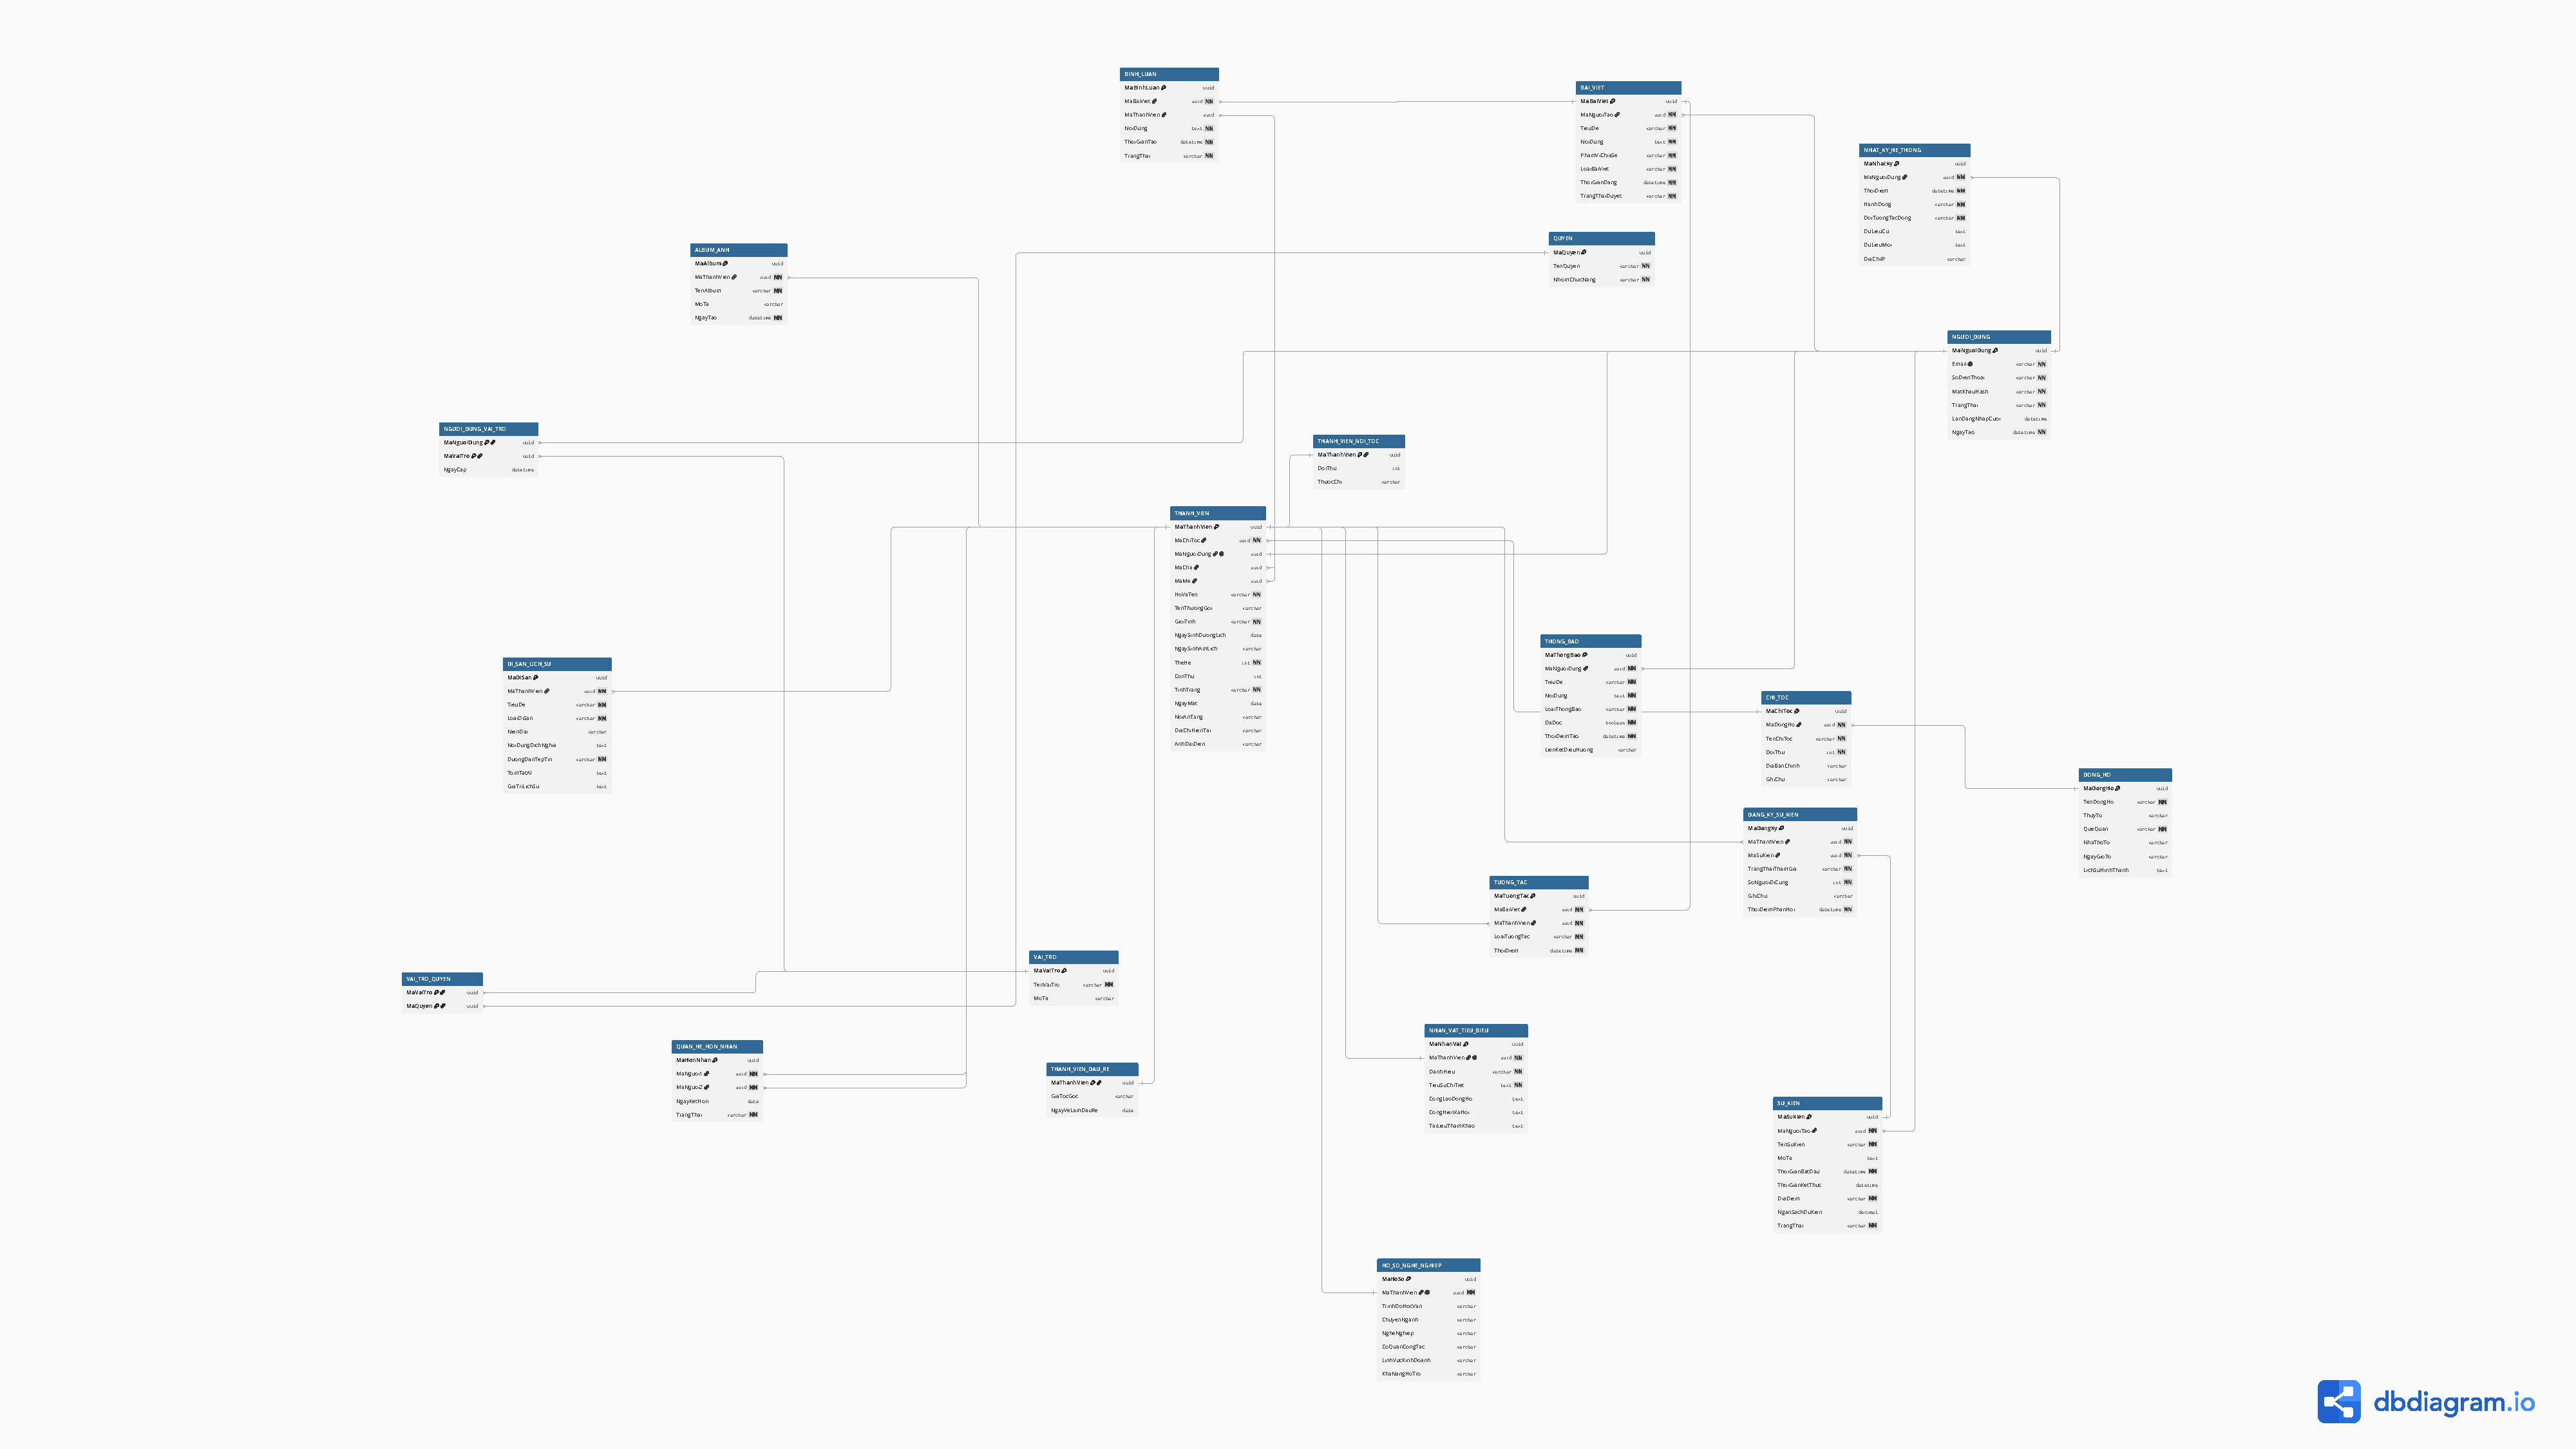
\includegraphics[page=1, trim={295pt 50pt 295pt 45pt}, clip, width=1.06\textwidth]{figures/erd_logic.pdf}%
    }
    \caption{Sơ đồ ERD ở mức Logic của hệ thống FamilyConnect (Toàn cảnh 22 bảng)}
    \label{fig:erd_logic_diagram}
\end{figure}

\noindent\textbf{Liên kết mô hình tương tác trực tuyến:} Nhằm hỗ trợ việc theo dõi chi tiết các trường, kiểu dữ liệu và mối liên kết trực quan giữa 22 bảng ở độ phân giải gốc cao nhất, sơ đồ được xuất bản trực tuyến tại: \url{https://dbdiagram.io/d/Test-6ab17faa9ba2420e18d44291}.

\subsection{Phân tích kiến trúc liên kết theo phân hệ nghiệp vụ}

Dựa trên sơ đồ ERD mức Logic (Hình~\ref{fig:erd_logic_diagram}), cấu trúc quan hệ giữa 22 bảng được tổ chức thành 4 phân hệ chức năng đồng bộ:

\subsubsection{1. Phân hệ Tài khoản, Xác thực \& Phân quyền RBAC}
\begin{itemize}
    \item \textbf{Bảng trung tâm:} \texttt{nguoi\_dung} (PK: \texttt{ma\_nguoi\_dung}) đóng vai trò quản lý tài khoản xác thực độc lập.
    \item \textbf{Phân quyền đa cấp ($M:N$):} Được tổ chức chặt chẽ thông qua hai bảng trung gian:
    \begin{itemize}
        \item Bảng \texttt{nguoi\_dung\_vai\_tro} lưu vết việc gán vai trò (\texttt{vai\_tro}) cho người dùng kèm mốc thời gian cấp (\texttt{ngay\_cap}).
        \item Bảng \texttt{vai\_tro\_quyen} phân rã các hành động nghiệp vụ chi tiết (\texttt{quyen}) cho từng vai trò cụ thể.
    \end{itemize}
    \item \textbf{Nhật ký kiểm toán:} Bảng \texttt{nhat\_ky\_he\_thong} liên kết trực tiếp với \texttt{nguoi\_dung} qua FK \texttt{ma\_nguoi\_dung} (\texttt{ON DELETE CASCADE}) để ghi vết mọi hoạt động truy cập và biến động dữ liệu.
\end{itemize}

\subsubsection{2. Phân hệ Cốt lõi: Gia tộc, Chi tộc \& Phả hệ Huyết thống}
\begin{itemize}
    \item \textbf{Cây tổ chức dòng họ:} Thiết lập phân cấp chặt chẽ $1:N$ từ \texttt{dong\_ho} $\to$ \texttt{chi\_toc} $\to$ \texttt{thanh\_vien}. Mọi thành viên bắt buộc phải thuộc về một chi tộc cụ thể.
    \item \textbf{Thực thể trung tâm \texttt{thanh\_vien}:} Là tâm điểm kết nối của toàn bộ cơ sở dữ liệu:
    \begin{itemize}
        \item Liên kết tùy chọn $1:1$ với tài khoản hệ thống: FK \texttt{ma\_nguoi\_dung} ($\to$ \texttt{nguoi\_dung}) phục vụ nghiệp vụ nhận hồ sơ gia phả cá nhân (\textit{Profile Claiming}).
        \item Quan hệ đệ quy huyết thống ($1:N$): Hai cột FK \texttt{ma\_cha} và \texttt{ma\_me} tự tham chiếu về chính \texttt{thanh\_vien.ma\_thanh\_vien} (\texttt{ON DELETE SET NULL}), hỗ trợ thuật toán duyệt cây gia phả nhiều thế hệ.
        \item Quan hệ hôn phối ($M:N$): Bảng trung gian \texttt{quan\_he\_hon\_nhan} chứa cặp FK (\texttt{ma\_nguoi1}, \texttt{ma\_nguoi2}) đều tham chiếu về \texttt{thanh\_vien}, lưu giữ trạng thái và mốc thời gian kết hôn lịch sử.
    \end{itemize}
    \item \textbf{Bảng kế thừa thực thể con ($1:1$):} Hai bảng \texttt{thanh\_vien\_}\allowbreak\texttt{noi\_toc} và \texttt{thanh\_vien\_}\allowbreak\texttt{dau\_re} dùng chung PK \texttt{ma\_thanh\_vien} đồng thời đóng vai trò là FK tham chiếu về bảng cha \texttt{thanh\_vien} (\texttt{CASCADE}), phân tách rành mạch thuộc tính riêng của người ruột thịt và dâu/rể.
    \item \textbf{Hồ sơ nghề nghiệp:} Bảng phụ \texttt{ho\_so\_nghe\_nghiep} gắn với \texttt{thanh\_vien} theo tỷ lệ $1:1$ bắt buộc thông qua ràng buộc \texttt{UNIQUE} trên FK \texttt{ma\_thanh\_vien}.
\end{itemize}

\subsubsection{3. Phân hệ Mạng xã hội Gia đình, Sự kiện \& Truyền thông}
\begin{itemize}
    \item \textbf{Bảng tin \& Tương tác:} Bảng \texttt{bai\_viet} nhận FK \texttt{ma\_nguoi\_tao} từ \texttt{nguoi\_dung}. Các phản hồi thảo luận được lưu ở bảng phụ \texttt{binh\_luan} (FK: \texttt{ma\_bai\_viet}). Tương tác cảm xúc được xử lý qua bảng trung gian \texttt{tuong\_tac} kết nối giữa \texttt{thanh\_vien} và \texttt{bai\_viet}.
    \item \textbf{Kho lưu trữ hình ảnh:} Bảng \texttt{album\_anh} trực thuộc quyền quản lý của thành viên gia đình thông qua FK \texttt{ma\_thanh\_vien}.
    \item \textbf{Tổ chức sự kiện \& Điểm danh RSVP:} Bảng \texttt{su\_kien} quản lý các buổi lễ giỗ, họp mặt gia tộc. Việc đăng ký tham dự được thực thể hóa qua bảng trung gian \texttt{dang\_ky\_su\_kien} chứa các cặp khóa ngoại (\texttt{ma\_thanh\_vien}, \texttt{ma\_su\_kien}) cùng số lượng người đi cùng và trạng thái điểm danh.
    \item \textbf{Thông báo đa kênh:} Bảng \texttt{thong\_bao} phụ thuộc tồn tại vào tài khoản người nhận (\texttt{nguoi\_dung}).
\end{itemize}

\subsubsection{4. Phân hệ Di sản số \& Vinh danh Tiền nhân}
\begin{itemize}
    \item \textbf{Di sản tư liệu lịch sử:} Bảng \texttt{di\_san\_lich\_su} lưu giữ các văn bản, gia phả cổ, sắc phong do thành viên tải lên (FK: \texttt{ma\_thanh\_vien}).
    \item \textbf{Vinh danh danh nhân gia tộc:} Bảng phụ \texttt{nhan\_vat\_tieu\_bieu} tôn vinh các tiền nhân có công trạng lớn, liên kết $1:1$ với \texttt{thanh\_vien} qua FK \texttt{ma\_thanh\_vien} mang ràng buộc \texttt{UNIQUE}.
\end{itemize}

\subsection{Đánh giá tính nhất quán và toàn vẹn của mô hình}

Sơ đồ ERD ở mức Logic thể hiện tính khoa học và chuẩn mực cao trong thiết kế CSDL quan hệ:
\begin{enumerate}
    \item \textbf{Bảo toàn phụ thuộc hàm và không mất mát thông tin:} Toàn bộ 17 thực thể nghiệp vụ ban đầu cùng các mối kết hợp được bảo toàn 100\% khi phân rã thành 22 quan hệ.
    \item \textbf{Triệt tiêu dư thừa dữ liệu:} Tất cả các bảng trung gian giải quyết dứt điểm các mối kết hợp nhiều--nhiều, không tồn tại thuộc tính lặp hay phụ thuộc bắc cầu, đảm bảo chuẩn hóa dữ liệu tối ưu.
    \item \textbf{Toàn vẹn tham chiếu chặt chẽ:} Thiết lập tường minh các chính sách hành vi ngoại vi (\texttt{CASCADE}, \texttt{SET NULL}, \texttt{RESTRICT}) giúp cơ sở dữ liệu duy trì tính ổn định, sẵn sàng chuyển giao sang giai đoạn Thiết kế Vật lý trên hệ quản trị CSDL (Chương~\ref{chap:chuong3_vat_ly}).
\end{enumerate}

